% Options for packages loaded elsewhere
\PassOptionsToPackage{unicode}{hyperref}
\PassOptionsToPackage{hyphens}{url}
%
\documentclass[
  ignorenonframetext,
]{beamer}
\usepackage{pgfpages}
\setbeamertemplate{caption}[numbered]
\setbeamertemplate{caption label separator}{: }
\setbeamercolor{caption name}{fg=normal text.fg}
\beamertemplatenavigationsymbolsempty
% Prevent slide breaks in the middle of a paragraph
\widowpenalties 1 10000
\raggedbottom
\usepackage{lmodern}
\usepackage{amssymb,amsmath}
\usepackage{ifxetex,ifluatex}
\ifnum 0\ifxetex 1\fi\ifluatex 1\fi=0 % if pdftex
  \usepackage[T1]{fontenc}
  \usepackage[utf8]{inputenc}
  \usepackage{textcomp} % provide euro and other symbols
\else % if luatex or xetex
  \usepackage{unicode-math}
  \defaultfontfeatures{Scale=MatchLowercase}
  \defaultfontfeatures[\rmfamily]{Ligatures=TeX,Scale=1}
\fi
\usetheme[]{CambridgeUS}
% Use upquote if available, for straight quotes in verbatim environments
\IfFileExists{upquote.sty}{\usepackage{upquote}}{}
\IfFileExists{microtype.sty}{% use microtype if available
  \usepackage[]{microtype}
  \UseMicrotypeSet[protrusion]{basicmath} % disable protrusion for tt fonts
}{}
\makeatletter
\@ifundefined{KOMAClassName}{% if non-KOMA class
  \IfFileExists{parskip.sty}{%
    \usepackage{parskip}
  }{% else
    \setlength{\parindent}{0pt}
    \setlength{\parskip}{6pt plus 2pt minus 1pt}}
}{% if KOMA class
  \KOMAoptions{parskip=half}}
\makeatother
\usepackage{xcolor}
\IfFileExists{xurl.sty}{\usepackage{xurl}}{} % add URL line breaks if available
\IfFileExists{bookmark.sty}{\usepackage{bookmark}}{\usepackage{hyperref}}
\hypersetup{
  pdftitle={Formal verification of Scala programs with Stainless},
  pdfauthor={Romain Ruetschi},
  hidelinks,
  pdfcreator={LaTeX via pandoc}}
\urlstyle{same} % disable monospaced font for URLs
\newif\ifbibliography
\usepackage{color}
\usepackage{fancyvrb}
\newcommand{\VerbBar}{|}
\newcommand{\VERB}{\Verb[commandchars=\\\{\}]}
\DefineVerbatimEnvironment{Highlighting}{Verbatim}{commandchars=\\\{\}}
% Add ',fontsize=\small' for more characters per line
\newenvironment{Shaded}{}{}
\newcommand{\AlertTok}[1]{\textcolor[rgb]{1.00,0.00,0.00}{\textbf{#1}}}
\newcommand{\AnnotationTok}[1]{\textcolor[rgb]{0.38,0.63,0.69}{\textbf{\textit{#1}}}}
\newcommand{\AttributeTok}[1]{\textcolor[rgb]{0.49,0.56,0.16}{#1}}
\newcommand{\BaseNTok}[1]{\textcolor[rgb]{0.25,0.63,0.44}{#1}}
\newcommand{\BuiltInTok}[1]{#1}
\newcommand{\CharTok}[1]{\textcolor[rgb]{0.25,0.44,0.63}{#1}}
\newcommand{\CommentTok}[1]{\textcolor[rgb]{0.38,0.63,0.69}{\textit{#1}}}
\newcommand{\CommentVarTok}[1]{\textcolor[rgb]{0.38,0.63,0.69}{\textbf{\textit{#1}}}}
\newcommand{\ConstantTok}[1]{\textcolor[rgb]{0.53,0.00,0.00}{#1}}
\newcommand{\ControlFlowTok}[1]{\textcolor[rgb]{0.00,0.44,0.13}{\textbf{#1}}}
\newcommand{\DataTypeTok}[1]{\textcolor[rgb]{0.56,0.13,0.00}{#1}}
\newcommand{\DecValTok}[1]{\textcolor[rgb]{0.25,0.63,0.44}{#1}}
\newcommand{\DocumentationTok}[1]{\textcolor[rgb]{0.73,0.13,0.13}{\textit{#1}}}
\newcommand{\ErrorTok}[1]{\textcolor[rgb]{1.00,0.00,0.00}{\textbf{#1}}}
\newcommand{\ExtensionTok}[1]{#1}
\newcommand{\FloatTok}[1]{\textcolor[rgb]{0.25,0.63,0.44}{#1}}
\newcommand{\FunctionTok}[1]{\textcolor[rgb]{0.02,0.16,0.49}{#1}}
\newcommand{\ImportTok}[1]{#1}
\newcommand{\InformationTok}[1]{\textcolor[rgb]{0.38,0.63,0.69}{\textbf{\textit{#1}}}}
\newcommand{\KeywordTok}[1]{\textcolor[rgb]{0.00,0.44,0.13}{\textbf{#1}}}
\newcommand{\NormalTok}[1]{#1}
\newcommand{\OperatorTok}[1]{\textcolor[rgb]{0.40,0.40,0.40}{#1}}
\newcommand{\OtherTok}[1]{\textcolor[rgb]{0.00,0.44,0.13}{#1}}
\newcommand{\PreprocessorTok}[1]{\textcolor[rgb]{0.74,0.48,0.00}{#1}}
\newcommand{\RegionMarkerTok}[1]{#1}
\newcommand{\SpecialCharTok}[1]{\textcolor[rgb]{0.25,0.44,0.63}{#1}}
\newcommand{\SpecialStringTok}[1]{\textcolor[rgb]{0.73,0.40,0.53}{#1}}
\newcommand{\StringTok}[1]{\textcolor[rgb]{0.25,0.44,0.63}{#1}}
\newcommand{\VariableTok}[1]{\textcolor[rgb]{0.10,0.09,0.49}{#1}}
\newcommand{\VerbatimStringTok}[1]{\textcolor[rgb]{0.25,0.44,0.63}{#1}}
\newcommand{\WarningTok}[1]{\textcolor[rgb]{0.38,0.63,0.69}{\textbf{\textit{#1}}}}
\usepackage{graphicx,grffile}
\makeatletter
\def\maxwidth{\ifdim\Gin@nat@width>\linewidth\linewidth\else\Gin@nat@width\fi}
\def\maxheight{\ifdim\Gin@nat@height>\textheight\textheight\else\Gin@nat@height\fi}
\makeatother
% Scale images if necessary, so that they will not overflow the page
% margins by default, and it is still possible to overwrite the defaults
% using explicit options in \includegraphics[width, height, ...]{}
\setkeys{Gin}{width=\maxwidth,height=\maxheight,keepaspectratio}
% Set default figure placement to htbp
\makeatletter
\def\fps@figure{htbp}
\makeatother
\setlength{\emergencystretch}{3em} % prevent overfull lines
\providecommand{\tightlist}{%
  \setlength{\itemsep}{0pt}\setlength{\parskip}{0pt}}
\setcounter{secnumdepth}{-\maxdimen} % remove section numbering
\institute{Laboratory for Automated Reasoning and Analysis, EPFL}
\useinnertheme{rectangles}
\useoutertheme{infolines}
\definecolor{darkred}{rgb}{0.8,0,0}
\usecolortheme[named=darkred]{structure}
\setbeamertemplate{footline}{frame number}
\setbeamertemplate{navigation symbols}{}
\setbeamertemplate{footline}{}
\usepackage[]{biblatex}
\addbibresource{slides.bib}

\title{Formal verification of Scala programs with Stainless}
\author{Romain Ruetschi}
\date{Typelevel Summit Lausanne 2019}

\begin{document}
\frame{\titlepage}

\begin{frame}{About me}
\protect\hypertarget{about-me}{}

\begin{itemize}
\tightlist
\item
  Romain Ruetschi (Romac)
\item
  MSc in Computer Science from EPFL
\item
  \textasciitilde2 years as an engineer at LARA
\end{itemize}

\end{frame}

\begin{frame}{Outline}
\protect\hypertarget{outline}{}

\begin{itemize}
\tightlist
\item
  Stainless: Verification framework for Scala
\item
  What Stainless verifies
\item
  Termination checker
\item
  Case study: Verifying typeclasses
\item
  More case studies
\item
  Bonus
\item
  Coming soon / further work
\end{itemize}

\end{frame}

\begin{frame}{Stainless: Verification framework for Scala}
\protect\hypertarget{stainless-verification-framework-for-scala}{}

Stainless is a verification framework for higher-order programs written
in a subset of Scala, named \emph{PureScala}:

\begin{itemize}
\tightlist
\item
  Traits, abstract classes, case classes, implicit classes, methods
\item
  Higher-order functions, lambdas
\item
  Any, Nothing, co-/contra-variant type parameters
\item
  Single inheritance
\item
  Anonymous and local classes, inner functions
\end{itemize}

\end{frame}

\begin{frame}[fragile]

\begin{itemize}
\tightlist
\item
  Type members, type aliases
\item
  GADTs
\item
  \texttt{PartialFunction}s
\item
  Set, Bag, List, Map, Array, Byte, Short, Int, Long, BigInt
\item
  Local state, \texttt{while}, traits/classes with \texttt{var}s, and
  more\ldots{}
\end{itemize}

Currently supports Scala 2.12.x.

\end{frame}

\begin{frame}

Some Dotty-specific features:

\begin{itemize}
\tightlist
\item
  Intersection and union types
\item
  Dependent function types
\item
  Extension methods
\item
  Opaque types
\end{itemize}

Currently only supports Dotty 0.12.0, will try to catch up.

\end{frame}

\begin{frame}[fragile]{What Stainless verifies}
\protect\hypertarget{what-stainless-verifies}{}

\begin{itemize}
\tightlist
\item
  \textbf{Assertions} which should hold at the place where they are
  stated, \textbf{checked statically}
\item
  \textbf{Postconditions} using \texttt{ensuring} function: assertions
  for return values of functions
\item
  \textbf{Preconditions} using \texttt{require} function: assertions on
  function parameters
\item
  \textbf{Loop invariants}: inductive assertions that hold in each loop
  iteration after the while condition check passes
\item
  \textbf{ADT/Class invariants}: assertions on constructors parameters
  (which remain true for all constructed values)
\end{itemize}

\end{frame}

\begin{frame}

Stainless also automatically performs \textbf{automatic checks for the
absence of runtime failures}:

\begin{itemize}
\tightlist
\item
  Exhaustiveness of pattern matching (taking guards into account)
\item
  Division by zero, array bounds checks
\item
  Map domain checks
\end{itemize}

\end{frame}

\begin{frame}

Moreover, Stainless also prevents \emph{PureScala} programs from:

\begin{itemize}
\tightlist
\item
  Creating null values or unininitalized local variables or fields
\item
  Explicitly throwing an exception
\item
  Overflows and underflows on sized integer types
\end{itemize}

\end{frame}

\begin{frame}{Termination checker}
\protect\hypertarget{termination-checker}{}

A \emph{verified} function in stainless is guaranteed to never crash,
however, it can still lead to an infinite evaluation.

Stainless therefore provides a termination checker that complements the
verification of safety properties.

\end{frame}

\begin{frame}{Pipeline}
\protect\hypertarget{pipeline}{}

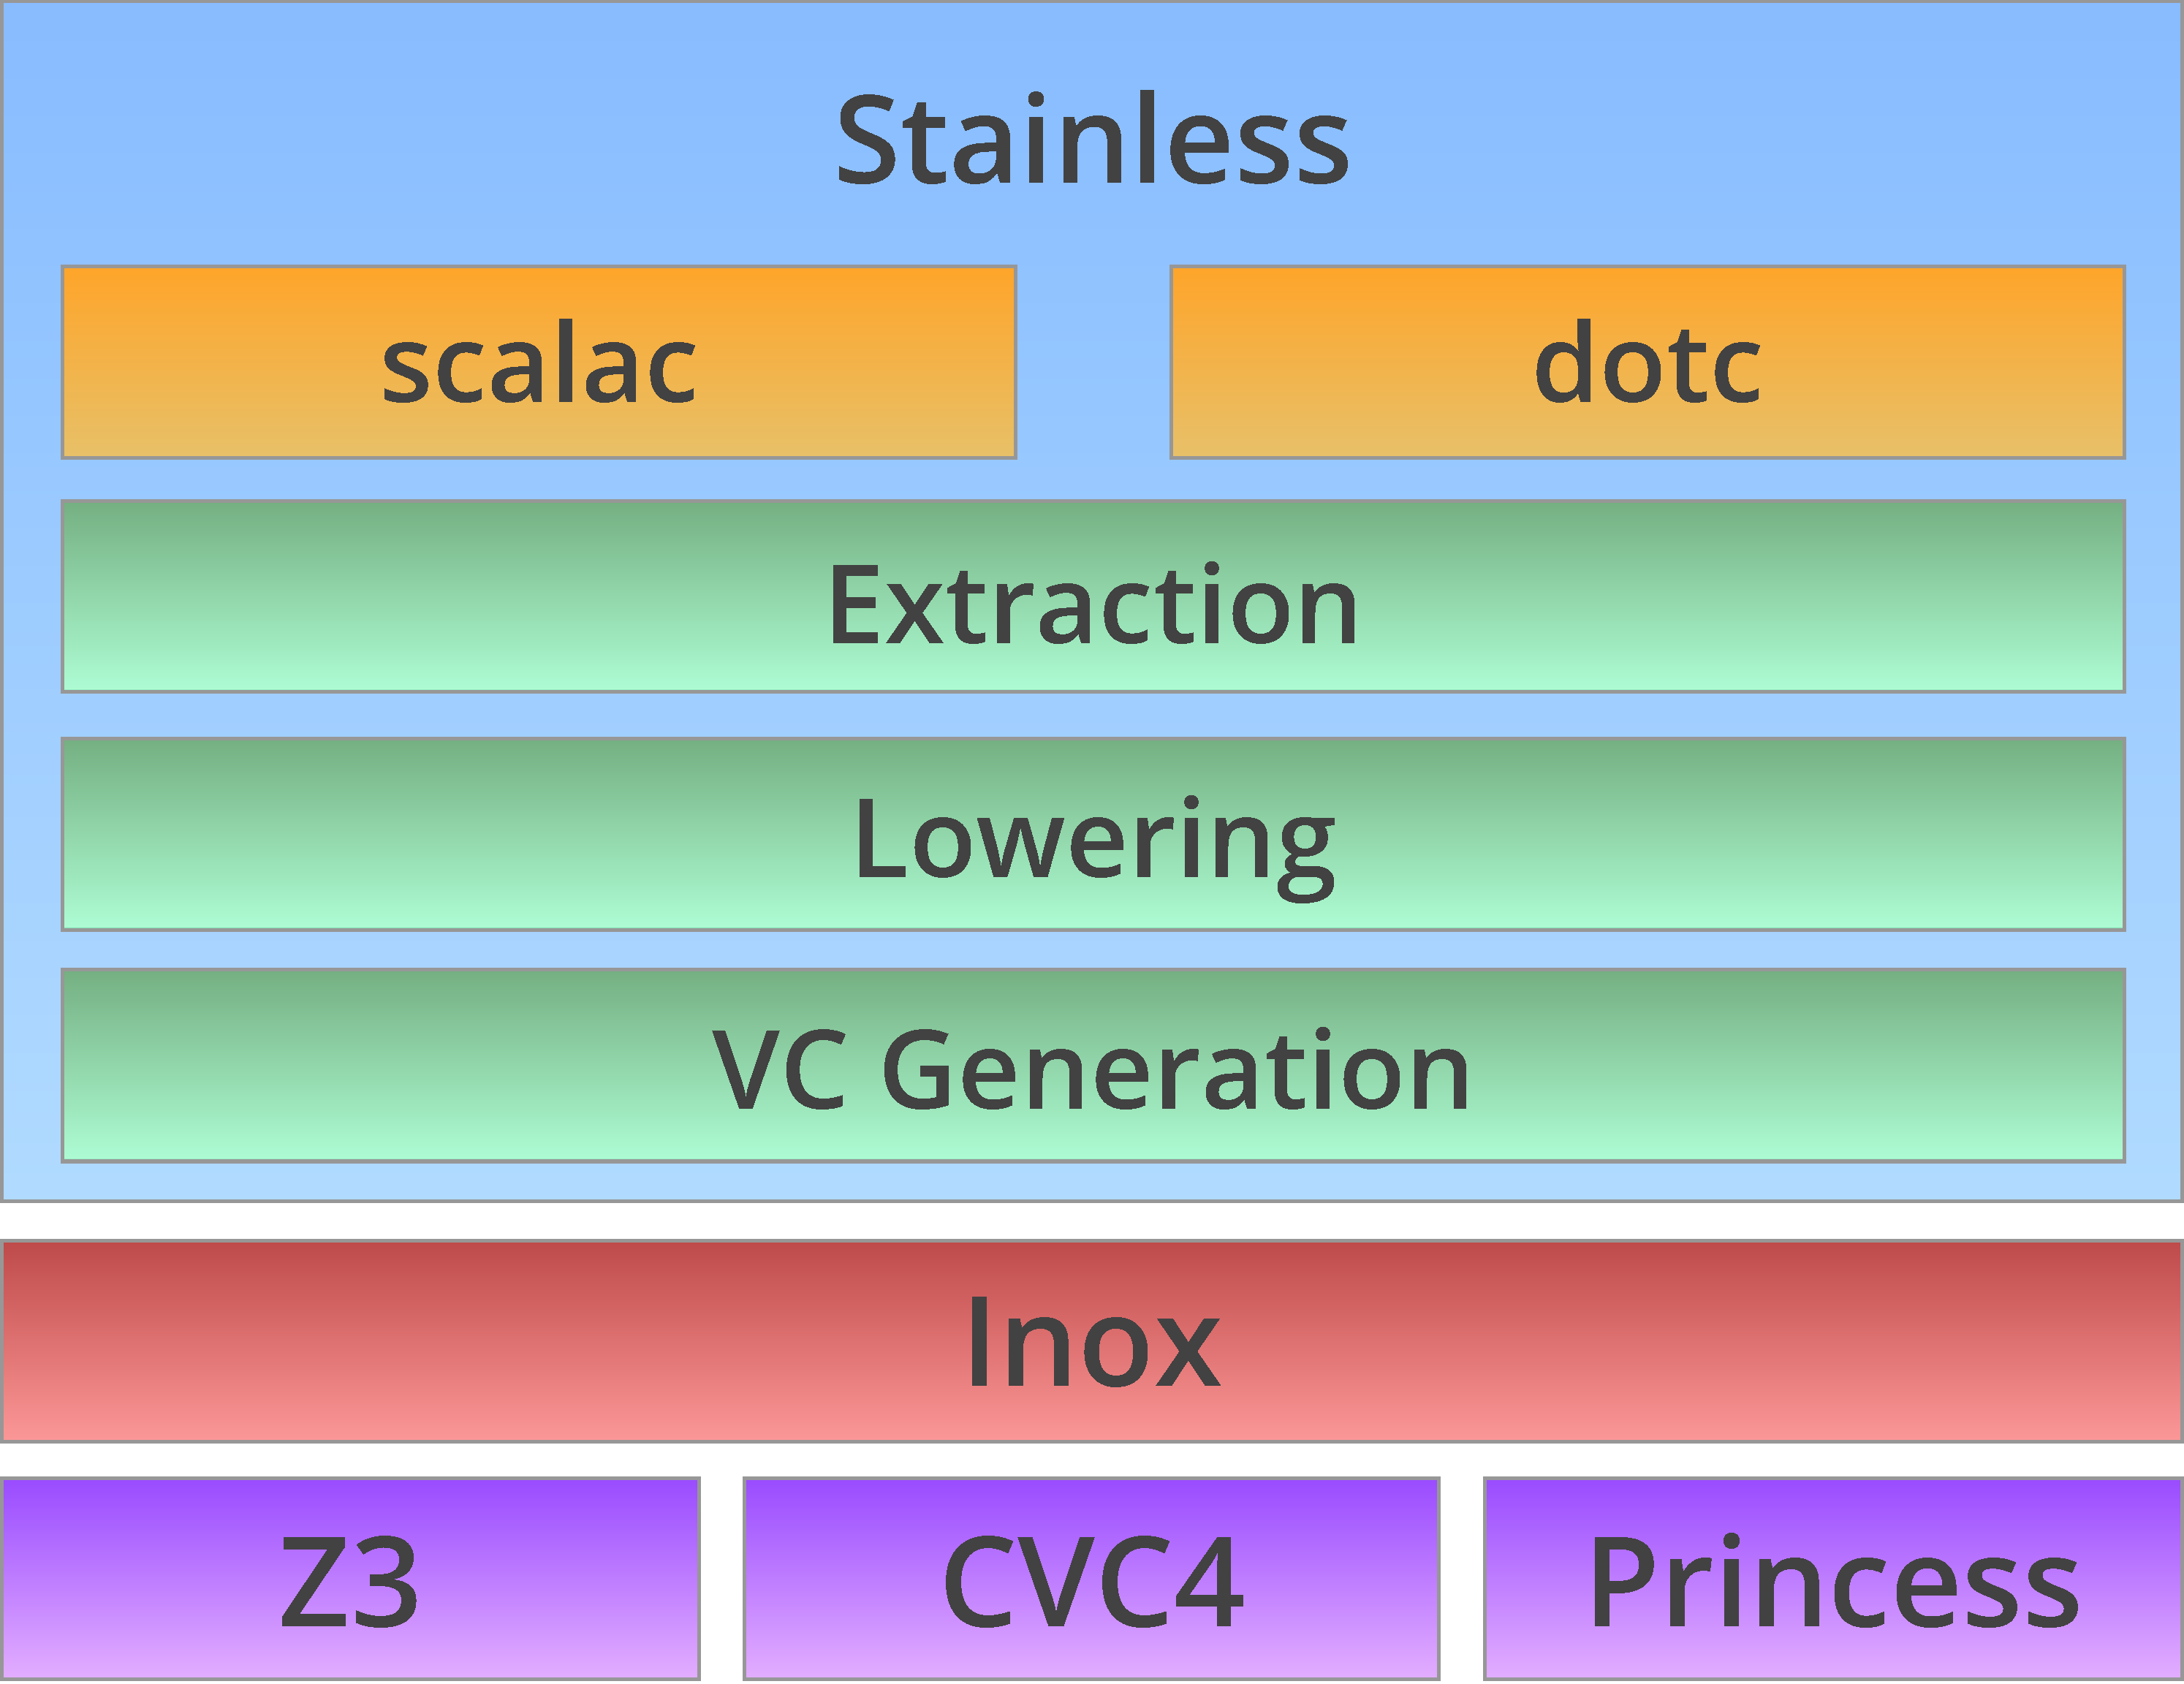
\includegraphics[width=\textwidth,height=0.85\textheight]{stainless.pdf}

\end{frame}

\begin{frame}[fragile]{Case study: Verifying typeclasses}
\protect\hypertarget{case-study-verifying-typeclasses}{}

\begin{Shaded}
\begin{Highlighting}[]
\NormalTok{Seq(}\DecValTok{1}\NormalTok{, }\DecValTok{2}\NormalTok{, }\DecValTok{3}\NormalTok{, }\DecValTok{4}\NormalTok{).}\FunctionTok{par}\NormalTok{.}\FunctionTok{fold}\NormalTok{(}\DecValTok{10}\NormalTok{)(_ - _)}

\CommentTok{// ((((10 - 1) - 2) - 3) - 4) => 0}
\CommentTok{// (10 - 1) - (2 - (3 - 4))   => 6}
\end{Highlighting}
\end{Shaded}

\end{frame}

\begin{frame}[fragile]

\begin{Shaded}
\begin{Highlighting}[]
\NormalTok{Seq(}\DecValTok{1}\NormalTok{, }\DecValTok{2}\NormalTok{, }\DecValTok{3}\NormalTok{, }\DecValTok{4}\NormalTok{).}\FunctionTok{par}\NormalTok{.}\FunctionTok{fold}\NormalTok{(}\DecValTok{0}\NormalTok{)(_ + _)}

\CommentTok{// ((((10 + 1) + 2) + 3) + 4) => 10}
\CommentTok{// (10 + 1) + (2 + (3 + 4))   => 10}
\end{Highlighting}
\end{Shaded}

\end{frame}

\begin{frame}[fragile]

\begin{Shaded}
\begin{Highlighting}[]
\KeywordTok{abstract} \KeywordTok{class}\NormalTok{ Semigroup[A] \{}
  \KeywordTok{def} \FunctionTok{combine}\NormalTok{(x: A, y: A): A}

\NormalTok{  @law }\KeywordTok{def} \FunctionTok{law_assoc}\NormalTok{(x: A, y: A, z: A) =}
    \FunctionTok{combine}\NormalTok{(x, }\FunctionTok{combine}\NormalTok{(y, z)) == }\FunctionTok{combine}\NormalTok{(}\FunctionTok{combine}\NormalTok{(x, y), z)}
\NormalTok{\}}
\end{Highlighting}
\end{Shaded}

\end{frame}

\begin{frame}[fragile]

\begin{Shaded}
\begin{Highlighting}[]
\KeywordTok{abstract} \KeywordTok{class}\NormalTok{ Monoid[A]}
  \KeywordTok{extends}\NormalTok{ Semigroup[A] \{}

  \KeywordTok{def}\NormalTok{ empty: A}

\NormalTok{  @law }\KeywordTok{def} \FunctionTok{law_leftIdentity}\NormalTok{(x: A) =}
    \FunctionTok{combine}\NormalTok{(empty, x) == x}

\NormalTok{  @law }\KeywordTok{def} \FunctionTok{law_rightIdentity}\NormalTok{(x: A) =}
    \FunctionTok{combine}\NormalTok{(x, empty) == x}
\NormalTok{\}}
\end{Highlighting}
\end{Shaded}

\end{frame}

\begin{frame}[fragile]

\begin{Shaded}
\begin{Highlighting}[]
\KeywordTok{case} \KeywordTok{class} \FunctionTok{Sum}\NormalTok{(get: BigInt)}

\KeywordTok{implicit} \KeywordTok{def}\NormalTok{ sumMonoid = }\KeywordTok{new}\NormalTok{ Monoid[Sum] \{}
  \KeywordTok{def}\NormalTok{ empty = }\FunctionTok{Sum}\NormalTok{(}\DecValTok{0}\NormalTok{)}
  \KeywordTok{def} \FunctionTok{combine}\NormalTok{(x: Sum, y: Sum) = }\FunctionTok{Sum}\NormalTok{(x.}\FunctionTok{get}\NormalTok{ + y.}\FunctionTok{get}\NormalTok{)}
\NormalTok{\}}
\end{Highlighting}
\end{Shaded}

\end{frame}

\begin{frame}[fragile]

\begin{Shaded}
\begin{Highlighting}[]
\KeywordTok{val}\NormalTok{ A: (Object) => Boolean = (x: Object) => x is Sum}
\KeywordTok{val}\NormalTok{ x: \{ x: Object | @unchecked }\FunctionTok{A}\NormalTok{(x) \} = }\FunctionTok{Sum}\NormalTok{(x)}
\KeywordTok{val}\NormalTok{ y: \{ x: Object | @unchecked }\FunctionTok{A}\NormalTok{(x) \} = }\FunctionTok{Sum}\NormalTok{(y)}
\KeywordTok{val}\NormalTok{ z: \{ x: Object | @unchecked }\FunctionTok{A}\NormalTok{(x) \} = }\FunctionTok{Sum}\NormalTok{(z)}

\KeywordTok{val}\NormalTok{ res: Boolean = \{}
  \FunctionTok{combine}\NormalTok{(A, thiss, x, }\FunctionTok{combine}\NormalTok{(A, thiss, y, z)) ==}
  \FunctionTok{combine}\NormalTok{(A, thiss, }\FunctionTok{combine}\NormalTok{(A, thiss, x, y), z)}
\NormalTok{\}}

\FunctionTok{assume}\NormalTok{(res == }\FunctionTok{law_assoc}\NormalTok{(thiss, x, y, z))}

\NormalTok{res}
\end{Highlighting}
\end{Shaded}

\end{frame}

\begin{frame}[fragile]

\begin{verbatim}
  ┌───────────────────┐
╔═╡ stainless summary ╞═══════════════════════════════════╗
║ └───────────────────┘                                   ║
║ law_leftIdentity    law   valid   nativez3   0.223      ║
║ law_rightIdentity   law   valid   nativez3   0.407      ║
║ law_assoc           law   valid   nativez3   0.944      ║
╟┄┄┄┄┄┄┄┄┄┄┄┄┄┄┄┄┄┄┄┄┄┄┄┄┄┄┄┄┄┄┄┄┄┄┄┄┄┄┄┄┄┄┄┄┄┄┄┄┄┄┄┄┄┄┄┄┄╢
║ total: 3  valid: 3  invalid: 0  unknown: 0  time: 1.574 ║
╚═════════════════════════════════════════════════════════╝
\end{verbatim}

\end{frame}

\begin{frame}[fragile]

\begin{Shaded}
\begin{Highlighting}[]
\KeywordTok{implicit} \KeywordTok{def}\NormalTok{ optionMonoid[A](}\KeywordTok{implicit}\NormalTok{ S: Semigroup[A]) =}
  \KeywordTok{new}\NormalTok{ Monoid[Option[A]] \{}
    \KeywordTok{def}\NormalTok{ empty: Option[A] = None()}

    \KeywordTok{def} \FunctionTok{combine}\NormalTok{(x: Option[A], y: Option[A]) =}
\NormalTok{      x }\KeywordTok{match}\NormalTok{ \{}
        \KeywordTok{case}\NormalTok{ None()   => y}
        \KeywordTok{case}\NormalTok{ Some(xv) => y }\KeywordTok{match}\NormalTok{ \{}
          \KeywordTok{case}\NormalTok{ None()   => x}
          \KeywordTok{case}\NormalTok{ Some(yv) => Some(S.}\FunctionTok{combine}\NormalTok{(xv, yv))}
\NormalTok{        \}}
\NormalTok{      \}}
\NormalTok{  \}}
\end{Highlighting}
\end{Shaded}

\end{frame}

\begin{frame}[fragile]

\begin{Shaded}
\begin{Highlighting}[]
\KeywordTok{implicit} \KeywordTok{def}\NormalTok{ optionMonoid[A](}\KeywordTok{implicit} \KeywordTok{val}\NormalTok{ S: Semigroup[A]) =}
  \KeywordTok{new}\NormalTok{ Monoid[Option[A]] \{}
    \CommentTok{// ...}

    \KeywordTok{override} \KeywordTok{def} \FunctionTok{law_assoc}\NormalTok{(@induct x: Option[A], y: Option[A], z: Option[A]) =}
      \KeywordTok{super}\NormalTok{.}\FunctionTok{law_assoc}\NormalTok{(x, y, z) because \{}
\NormalTok{        (x, y, z) }\KeywordTok{match}\NormalTok{ \{}
          \KeywordTok{case}\NormalTok{ (Some(xv), Some(yv), Some(zv)) =>}
\NormalTok{            S.}\FunctionTok{law_assoc}\NormalTok{(xv, yv, zv)}

          \KeywordTok{case}\NormalTok{ _ => }\KeywordTok{true}
\NormalTok{        \}}
\NormalTok{      \}}
\NormalTok{  \}}
\end{Highlighting}
\end{Shaded}

\end{frame}

\begin{frame}[fragile]

\begin{Shaded}
\begin{Highlighting}[]
\KeywordTok{val}\NormalTok{ A: (Object) => Boolean = (x: Object) =>}
\NormalTok{  x is Option && isOption[Object](x.}\FunctionTok{value}\NormalTok{, A)}

\KeywordTok{val}\NormalTok{ x: \{ x: Object | @unchecked }\FunctionTok{A}\NormalTok{(x) \} = Option(x)}
\KeywordTok{val}\NormalTok{ y: \{ x: Object | @unchecked }\FunctionTok{A}\NormalTok{(x) \} = Option(y)}
\KeywordTok{val}\NormalTok{ z: \{ x: Object | @unchecked }\FunctionTok{A}\NormalTok{(x) \} = Option(z)}

\NormalTok{x is Some ==> \{}
\NormalTok{  (x, y, z) }\KeywordTok{match}\NormalTok{ \{}
    \KeywordTok{case}\NormalTok{ (Some(xv), Some(yv), Some(zv)) =>}
      \FunctionTok{law_assoc}\NormalTok{(A, thiss.}\FunctionTok{S}\NormalTok{, xv, yv, zv)}
    \KeywordTok{case}\NormalTok{ _ =>}
      \KeywordTok{true}
\NormalTok{  \} && \{}
    \KeywordTok{val}\NormalTok{ res: Boolean = \{}
      \FunctionTok{combine}\NormalTok{(A, thiss, x, }\FunctionTok{combine}\NormalTok{(A, thiss, y, z)) ==}
      \FunctionTok{combine}\NormalTok{(A, thiss, }\FunctionTok{combine}\NormalTok{(A, thiss, x, y), z)}
\NormalTok{    \}}
    \FunctionTok{assume}\NormalTok{(res == }\FunctionTok{law_assoc}\NormalTok{(thiss, x, y, z))}
\NormalTok{    res}
\NormalTok{  \}}
\NormalTok{\}}
\end{Highlighting}
\end{Shaded}

\end{frame}

\begin{frame}[fragile]

\begin{Shaded}
\begin{Highlighting}[]
\NormalTok{x$}\DecValTok{569}\NormalTok{ is None$}\DecValTok{0}\NormalTok{ ==> \{}
  \CommentTok{// snip...}
\NormalTok{\}}
\end{Highlighting}
\end{Shaded}

\end{frame}

\begin{frame}[fragile]

\begin{Shaded}
\begin{Highlighting}[]
\KeywordTok{def}\NormalTok{ foldMap[M, A](xs: List[A])(f: A => M)(}\KeywordTok{implicit}\NormalTok{ M: Monoid[A]): M =}
\NormalTok{  xs.}\FunctionTok{map}\NormalTok{(f).}\FunctionTok{fold}\NormalTok{(M.}\FunctionTok{empty}\NormalTok{)(M.}\FunctionTok{append}\NormalTok{)}

\NormalTok{@extern}
\KeywordTok{def}\NormalTok{ parFoldMap[M, A](xs: List[A])(f: A => M)(}\KeywordTok{implicit}\NormalTok{ M: Monoid[A]): M = \{}
\NormalTok{  xs.}\FunctionTok{toScala}\NormalTok{.}\FunctionTok{par}\NormalTok{.}\FunctionTok{map}\NormalTok{(f).}\FunctionTok{fold}\NormalTok{(M.}\FunctionTok{empty}\NormalTok{)(M.}\FunctionTok{append}\NormalTok{)}
\NormalTok{\} ensuring \{ res =>}
\NormalTok{  res == }\FunctionTok{foldMap}\NormalTok{(xs, f)}
\NormalTok{\}}
\end{Highlighting}
\end{Shaded}

\end{frame}

\begin{frame}{More case studies}
\protect\hypertarget{more-case-studies}{}

\end{frame}

\begin{frame}{Conc-Rope}
\protect\hypertarget{conc-rope}{}

Verified data-structure which provides

\begin{itemize}
\tightlist
\item
  Worst-case \(O(log n)\) time lookup, update, split and concatenation
  operations
\item
  Amortized O(1) time append and prepend operations
\end{itemize}

Very useful for efficient data-parellel operations!

{[}ConcRope{]} TODO: Ref

\end{frame}

\begin{frame}{Parellel Map-Reduce pipeline}
\protect\hypertarget{parellel-map-reduce-pipeline}{}

Fully verified implementation of the previous running example, using a
Conc-Rope under the hood instead of Scala's `par' operator.

Built by Lucien Iseli, BSc student, as a semester project. TODO:
Benchmarks

\end{frame}

\begin{frame}[fragile]{Actor systems}
\protect\hypertarget{actor-systems}{}

\begin{Shaded}
\begin{Highlighting}[]
\KeywordTok{case} \KeywordTok{class} \FunctionTok{Primary}\NormalTok{(backup: ActorRef, counter: BigInt) }\KeywordTok{extends}\NormalTok{ Behavior \{}
  \KeywordTok{def} \FunctionTok{processMsg}\NormalTok{(msg: Msg): Behavior = msg }\KeywordTok{match}\NormalTok{ \{}
    \KeywordTok{case}\NormalTok{ Inc =>}
\NormalTok{      backup ! Inc}
      \FunctionTok{PrimBehav}\NormalTok{(backup, counter + }\DecValTok{1}\NormalTok{)}

    \KeywordTok{case}\NormalTok{ _ => }\KeywordTok{this}
\NormalTok{  \}}
\NormalTok{\}}
\end{Highlighting}
\end{Shaded}

\end{frame}

\begin{frame}[fragile]

\begin{Shaded}
\begin{Highlighting}[]
\KeywordTok{case} \KeywordTok{class} \FunctionTok{Backup}\NormalTok{(counter: BigInt) }\KeywordTok{extends}\NormalTok{ Behavior \{}
  \KeywordTok{def} \FunctionTok{processMsg}\NormalTok{(msg: Msg): Behavior = msg }\KeywordTok{match}\NormalTok{ \{}
    \KeywordTok{case}\NormalTok{ Inc => }\FunctionTok{BackBehav}\NormalTok{(counter + }\DecValTok{1}\NormalTok{)}
    \KeywordTok{case}\NormalTok{ _   => }\KeywordTok{this}
\NormalTok{  \}}
\NormalTok{\}}
\end{Highlighting}
\end{Shaded}

\end{frame}

\begin{frame}[fragile]

\begin{Shaded}
\begin{Highlighting}[]
\KeywordTok{def} \FunctionTok{invariant}\NormalTok{(s: ActorSystem): Boolean =}
  \KeywordTok{val}\NormalTok{ primary = s.}\FunctionTok{behaviors}\NormalTok{(PrimaryRef)}
  \KeywordTok{val}\NormalTok{ backup  = s.}\FunctionTok{behaviors}\NormalTok{(BackupRef)}
  \KeywordTok{val}\NormalTok{ pending = s.}\FunctionTok{inboxes}\NormalTok{(PrimaryRef -> BackupRef).}\FunctionTok{length}

\NormalTok{  primary.}\FunctionTok{counter}\NormalTok{ == backup.}\FunctionTok{counter}\NormalTok{ + pending}
\NormalTok{\}}
\end{Highlighting}
\end{Shaded}

\end{frame}

\begin{frame}[fragile]

\begin{Shaded}
\begin{Highlighting}[]
\KeywordTok{def} \FunctionTok{preserveInv}\NormalTok{(s: ActorSystem, n: ActorRef, m: ActorRef) = \{}
  \FunctionTok{require}\NormalTok{(}\FunctionTok{invariant}\NormalTok{(s))}

  \KeywordTok{val}\NormalTok{ next = s.}\FunctionTok{step}\NormalTok{(n, m)}

  \FunctionTok{invariant}\NormalTok{(next)}
\NormalTok{\}.}\FunctionTok{holds}
\end{Highlighting}
\end{Shaded}

\end{frame}

\begin{frame}[fragile]{Smart contracts}
\protect\hypertarget{smart-contracts}{}

We also maintain a fork of Stainless, called \emph{Smart} which
supports:

\begin{itemize}
\tightlist
\item
  Writing smart contracts in Scala
\item
  Specifying and proving properties of such programs, including precise
  reasoning about the \texttt{Uint256} data type
\item
  Generating Solidity source code from Scala, which can then be compiled
  and deployed using the usual tools for the Ethereum software ecosystem
\end{itemize}

{[}0{]} https://github.com/epfl-lara/smart

\end{frame}

\begin{frame}[fragile]{Bonus: Refinement types}
\protect\hypertarget{bonus-refinement-types}{}

\begin{Shaded}
\begin{Highlighting}[]
\KeywordTok{type}\NormalTok{ Nat = \{ n: BigInt => n >= }\FunctionTok{BigInt}\NormalTok{(}\DecValTok{0}\NormalTok{) \}}
\end{Highlighting}
\end{Shaded}

\end{frame}

\begin{frame}[fragile]

\begin{Shaded}
\begin{Highlighting}[]
\KeywordTok{def} \FunctionTok{sortedInsert}\NormalTok{(}
\NormalTok{  xs: \{ List[Int] => xs.}\FunctionTok{nonEmpty}\NormalTok{ \},}
\NormalTok{  x:  \{ Int => x <= xs.}\FunctionTok{head}\NormalTok{ \}}
\NormalTok{): \{ res: List[Int] => }\FunctionTok{isSorted}\NormalTok{(res) \} = \{}
\NormalTok{  x :: xs }\CommentTok{// VALID}
\NormalTok{\}}
\end{Highlighting}
\end{Shaded}

\end{frame}

\begin{frame}[fragile]{Bonus: Dependent function types}
\protect\hypertarget{bonus-dependent-function-types}{}

\begin{Shaded}
\begin{Highlighting}[]
\KeywordTok{trait}\NormalTok{ Entry \{}
  \KeywordTok{type}\NormalTok{ Key}
  \KeywordTok{val}\NormalTok{ key: Key}
\NormalTok{\}}

\KeywordTok{def} \FunctionTok{extractKey}\NormalTok{(e: Entry): e.}\FunctionTok{Key}\NormalTok{ = e.}\FunctionTok{key}

\KeywordTok{def}\NormalTok{ extractor: (e: Entry) => e.}\FunctionTok{Key}\NormalTok{ = }\FunctionTok{extractKey}\NormalTok{(_)}
\end{Highlighting}
\end{Shaded}

\end{frame}

\begin{frame}[fragile]

\begin{Shaded}
\begin{Highlighting}[]
\KeywordTok{case} \KeywordTok{class} \FunctionTok{IntEntry}\NormalTok{() }\KeywordTok{extends}\NormalTok{ Entry \{}
  \KeywordTok{type}\NormalTok{ Key = Int}
  \KeywordTok{val}\NormalTok{ key: Int = }\DecValTok{42}
\NormalTok{\}}

\FunctionTok{assert}\NormalTok{(}\FunctionTok{extractor}\NormalTok{(entry) == }\DecValTok{42}\NormalTok{) }\CommentTok{// VALID}
\end{Highlighting}
\end{Shaded}

\end{frame}

\begin{frame}{There is more!}
\protect\hypertarget{there-is-more}{}

\begin{itemize}
\tightlist
\item
  sbt plugin + metals integration
\item
  Ghost context (think Dotty's erased terms but more general)
\item
  Partial evaluation
\end{itemize}

\end{frame}

\begin{frame}{Coming soon(ish)}
\protect\hypertarget{coming-soonish}{}

\begin{itemize}
\tightlist
\item
  Higher-kinded types
\item
  Better support for refinement types and type members
\item
  VC generation via type-checking
\end{itemize}

\end{frame}

\begin{frame}{Coming later}
\protect\hypertarget{coming-later}{}

\begin{itemize}
\tightlist
\item
  Scala 2.13 / latest Dotty support
\item
  WebAssembly backend
\item
  and more\ldots{}
\end{itemize}

\end{frame}

\begin{frame}{Learn more}
\protect\hypertarget{learn-more}{}

\begin{itemize}
\tightlist
\item
  Installation
\item
  Tutorial
\item
  Ghost context
\item
  Imperative features
\item
  Working with existing code
\item
  Proving theorems
\item
  Stainless library
\item
  and more\ldots{}
\end{itemize}

=\textgreater{} \href{https://stainless.epfl.ch}{stainless.epfl.ch}

\end{frame}

\begin{frame}{Acknowledgments}
\protect\hypertarget{acknowledgments}{}

Stainless is the latest iteration of our verification system for Scala,
which was built and improved over time by many EPFL PhD students:
Nicolas Voirol, Jad Hamza, Régis Blanc, Eva Darulova, Etienne Kneuss,
Ravichandhran Kandhadai Madhavan, Mikaël Mayer, Emmanouil Koukoutos,
Ruzica Piskac, Philippe Suter, as well as Marco Antognini, Ivan Kuraj,
Lars Hupel, Samuel Grütter, and myself.

Many thanks as well to our friends at TripleQuote for their help with
the compiler and sbt plugins.

\end{frame}

\begin{frame}[allowframebreaks]{References}
  \bibliographytrue
  \printbibliography[heading=none]
\end{frame}

\end{document}
